% This work is licensed under the Creative Commons
% Attribution-NonCommercial-ShareAlike 4.0 International License. To view a copy
% of this license, visit http://creativecommons.org/licenses/by-nc-sa/4.0/ or
% send a letter to Creative Commons, PO Box 1866, Mountain View, CA 94042, USA.

% (c) Eric Kunze, 2019

%%%%%%%%%%%%%%%%%%%%%%%%%%%%%%%%%%%%%%%%%%%%%%%%%%%%%%%%%%%%%%%%%%%%%%%%%%%%
% Template for lecture notes and exercises at TU Dresden.
%%%%%%%%%%%%%%%%%%%%%%%%%%%%%%%%%%%%%%%%%%%%%%%%%%%%%%%%%%%%%%%%%%%%%%%%%%%%

\documentclass[ngerman, a4paper, 11pt]{article}

\usepackage[ngerman]{babel}
\usepackage[top=2.5cm,bottom=2.5cm,left=2.5cm,right=2.5cm]{geometry}
\usepackage{parskip}
\usepackage[onehalfspacing]{setspace} % increase row-space
\usepackage[utf8]{inputenc}

\usepackage{lmodern}
\usepackage{ulem} 

\usepackage{fancyhdr} 	% customize header / footer

\usepackage{amsmath,amssymb,amsfonts,mathtools}
%\usepackage{blkarray}
\usepackage{latexsym, marvosym, wasysym, stmaryrd}
\usepackage{bbm} 		% unitary matrix


% further support for different equation setting
\usepackage{cancel}
\usepackage{xfrac}		% sfrac -> fractions e.g. 3/4
\usepackage{diagbox}

\usepackage{../mathoperatorsLA}

\usepackage{tikz}
\usepackage{pgfplots}
\pgfplotsset{
	compat=1.10,% mit writeLaTeX bisher noch nicht möglich
	flaeche/.style={draw=none,fill=black,fill opacity=0.2},
	every axis/.append style={
		axis x line=middle,    % put the x axis in the middle
		axis y line=middle,    % put the y axis in the middle
		axis line style={->},  % arrows on the axis
	}
}
\usepackage{wrapfig}
\usepackage[table,dvipsnames]{tudscrcolor}
\usepackage{tabularx} 	% tabularx-environment (explicitly set width of columns)
\usepackage{multirow}
\usepackage{booktabs}	% improved rules


\newcommand{\begriff}[1]{\textbf{#1}}
\newcommand{\person}[1]{\textsc{#1}}

%%%%%%%%%%%%%%%%%%%%%%%%%%%%%%%%%%%%%%%%%%%%%%%%%%%%%%%%%%%%%%%%%%%
%                             COUNTER                             %
%%%%%%%%%%%%%%%%%%%%%%%%%%%%%%%%%%%%%%%%%%%%%%%%%%%%%%%%%%%%%%%%%%%
\usepackage{chngcntr}
\usepackage{enumerate}
\usepackage[inline]{enumitem} 		%customize label

\pretocmd{\chapter}{\setcounter{section}{0}}{}{}
\pretocmd{\chapter}{\setcounter{equation}{0}}{}{}

\renewcommand{\labelitemi}{\raisebox{2pt}{\scalebox{.4}{$\blacksquare$}}}
\renewcommand{\labelitemii}{$\vartriangleright$}
\renewcommand{\labelitemiii}{--}
% Variantionen des Dreiecks als Aufzählungszeichen $\blacktriangleright$ / $\vartriangleright$ / $\triangleright$

\renewcommand{\labelenumi}{(\arabic{enumi})}
\renewcommand{\labelenumii}{\alph{enumii}.}
\renewcommand{\labelenumiii}{\roman{enumiii}.}

%%%%%%%%%%%%%%%%%%%%%%%%%%%%%%%%%%%%%%%%%%%%%%%%%%%%%%%%%%%%%%%%%%%
\usepackage{titlesec}   % change title headings look
\usepackage{chngcntr}   % modify counters
\usepackage{relsize}    % relative font size (smaller[i], larger[i], ...)

\titleformat{\section}[hang]{\bfseries\LARGE\centering}{\thesection}{8pt}{}
%\titleformat*{\section}{\bfseries\titlefont\sectionsize}
\titleformat*{\subsection}{\sffamily\itshape\large\centering}

%%%%%%%%%%%%%%%%%%%%%%%%%%%%%%%%%%%%%%%%%%%%%%%%%%%%%%%%%%%%%%%%%%%

\usepackage{listings}
\lstdefinestyle{noframe}{
	basicstyle=\small\ttfamily,        % the size of the fonts that are used for the code
	breakatwhitespace=false,         % sets if automatic breaks should only happen at whitespace
	breaklines=true,                 % sets automatic line breaking
	commentstyle=\itshape,    	     % comment style
	escapeinside={\%*}{*)},          % if you want to add LaTeX within your code
	extendedchars=true,              % lets you use non-ASCII characters; for 8-bits encodings only, does not work with UTF-8
	firstnumber=1,                % start line enumeration with line 1000
	frame=none,
	keywordstyle=\bfseries,       % keyword style 
	language=Haskell,                 % the language of the code
	numbers=none,                    % where to put the line-numbers; possible: (none, left, right)
	tabsize=2,	                   % sets default tabsize to 2 spaces
}
\lstdefinestyle{frame}{
	basicstyle=\footnotesize\ttfamily,        % the size of the fonts that are used for the code
	breakatwhitespace=false,         % sets if automatic breaks should only happen at whitespace
	breaklines=true,                 % sets automatic line breaking
	commentstyle=\itshape,    	     % comment style
	escapeinside={\%*}{*)},          % if you want to add LaTeX within your code
	extendedchars=true,              % lets you use non-ASCII characters; for 8-bits encodings only, does not work with UTF-8
	firstnumber=1,                % start line enumeration with line 1000
	frame=single,
	keywordstyle=\bfseries,       % keyword style
	morekeywords={}, 
	language=Haskell,                 % the language of the code
	numbers=left,                    % where to put the line-numbers; possible: (none, left, right)
	numbersep=5pt,                   % how far the line-numbers are from the code
	numberstyle=\tiny\color{cdgray!50}, % the style that is used for the line-numbers
	rulecolor=\color{cddarkblue}, 
	tabsize=2,	                   % sets default tabsize to 2 spaces
}


%%%%%%%%%%%%%%%%%%%%%%%%%%%%%%%%%%%%%%%%%%%%%%%%%%%%%%%%%%%%%%%%%%%
% THEOREM ENVIRONMENTS // MATH

\usepackage{ntheorem}

\DeclareMathSymbol{*}{\mathbin}{symbols}{"01}

\counterwithin{equation}{section}
\newcounter{themcount}
\counterwithin{themcount}{section}

\newcommand{\skiparound}{10pt}
\theorempreskip{\skiparound}
\theorempostskip{\skiparound}

\theoremstyle{nonumberplain}
\theoremseparator{.}
\theorembodyfont{}

\newtheorem{aufgabe}{Aufgabe}
\newtheorem{beispiel}{Beispiel}
\theorembodyfont{\itshape}
\newtheorem{bemerkung}[themcount]{Bemerkung}

\usepackage[
	type={CC},
	modifier={by-nc-sa},
	version={4.0},
]{doclicense}

%%%%%%%%%%%%%%%%%%%%%%%%%%%%%%%%%%%%%%%%%%%%%%%%%%%%%%%%%%%%%%%%%%%
%                           REFERENCES                            %
%%%%%%%%%%%%%%%%%%%%%%%%%%%%%%%%%%%%%%%%%%%%%%%%%%%%%%%%%%%%%%%%%%%

\usepackage[unicode,bookmarks=true]{hyperref}
\hypersetup{
	% pdfborder={0 0 0}			% no boxed around links
	pdfborderstyle={/S/U/W 1},	% underlining insteas of boxes
	linkbordercolor=cdblue,
	urlbordercolor=cdblue
}

\usepackage{cleveref}
\crefname{bemerkung}{Bemerkung}{Bemerkungen}
\crefname{figure}{Abbildung}{Abbildungen}
\crefname{beispiel}{Beispiel}{Beispiele}

\usepackage{bookmark}		% pdf-bookmarks

%%%%%%%%%%%%%%%%%%%%%%%%%%%%%%%%%%%%%%%%%%%%%%%%%%%%%%%%%%%%%%%%%%%
%                      ADDITIONAL COMMANDS                        %
%%%%%%%%%%%%%%%%%%%%%%%%%%%%%%%%%%%%%%%%%%%%%%%%%%%%%%%%%%%%%%%%%%%

\newcommand*\ruleline[1]{\par\noindent\raisebox{.8ex}{\makebox[\linewidth]{\hrulefill\hspace{1ex}\raisebox{-.8ex}{#1}\hspace{1ex}\hrulefill}}}

\usepackage{opensans}
\usepackage{tcolorbox}
\usepackage[labelfont=bf, textfont=it]{caption}

% \usepackage[autostyle=true,german=quotes]{csquotes}
\newcommand*{\enq}[1]{\flq \ \!\!\! #1 \!\!\! \frq}

\renewcommand{\i}{i}

\begin{document}
	\begin{center}
		{\bfseries \sffamily \huge Umrechnung von Komplexen Zahlen} 
		
		\ruleline{\sffamily \Large Übungsblatt 1}
		
		{\scshape Eric Kunze --- \today}
	\end{center}
	\medskip
	
	{ \footnotesize \doclicenseThis }
	
	\begin{center}
		\small \slshape Keine Garantie auf Vollständigkeit und/oder Korrektheit!
	\end{center}
	
	Wie wir bereits gesehen haben, lassen sich komplexe Zahlen in arithmetischer Darstellung gut addieren und subtrahieren, allerdings wird es bei Multiplikation schon deutlich schwieriger. Für diese Operationen eignet sich die Exponentialform oder Polarkoordinaten deutlich besser. Wir wollen uns daher im Folgenden mit den Umrechnungen zwischen den verschiedenen Darstellungsformen beschäftigen. Zur Wiederholung aus der Vorlesung:
	
	\begin{tcolorbox}[colback=cdblue!10,colframe=cdblue]
		Sei $z \in \CC$ eine komplexe Zahl. Ihr Abstand vom Ursprung ist $r = \abs{z}$ und ihr \enquote{Öffnungswinkel} ist $\phi = \Arg(z)$.
		\begin{align*}
			z &= a + b \i \qquad (a,b \in \R) 
			\tag{arithmetische Darstellung} \\
			z &= r * e^{\i \phi}  
			\tag{\textsc{Euler}sche Darstellung} \\
			z &= r * \brackets{ \cos(\phi) + \i \sin(\phi)}
			\tag{trigonometrische Darstellung}
		\end{align*}
	\end{tcolorbox}
	
	Die beiden letzeren Darstellungen nutzen sogenannte Polarkoordinaten bestehend aus einem Radius $r \ge 0$ und einem Winkel $\phi$. Der Winkel soll zwischen $0$ und $2\pi$ liegen, d.h. $0 \le \phi < 2\pi$ erfüllen. 
	
	Wir können eine komplexe Zahl in der \textsc{Gauß}schen Zahlenebene darstellen (siehe \cref{fig: complex-plane}). Dort lassen sich die Parameter $a$ und $b$ aus der arithmetischen Darstellung als Koordinaten des Punktes in der Ebene interpretieren, aber auch $r$ und $\phi$ erkennen wir wieder. Weiter sehen wir mit den elementaren Sinus- und Kosinusfunktionen am rechtwinkligen Dreieck auch einen Zusammenhang zwischen den Koordinaten $(a,b)$ und $(r,\phi)$ (siehe dazu auch Gleichung \eqref{eq: sin-cos}).
	
	\begin{center}
		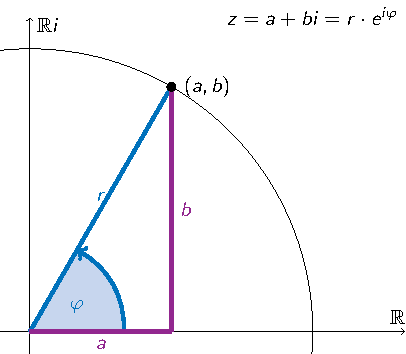
\includegraphics[scale=1]{complex-plane}
		\captionof{figure}{Koordinaten von komplexen Zahlen in der komplexen Ebene}
		\label{fig: complex-plane}
	\end{center}
	
	\section*{Polarkoordinaten $\to$ Arithmetische Darstellung}
	
	Sei unsere komplexe Zahl $z \in \CC$ gegeben in Polarkoordinaten, d.h. in der Form
	\begin{equation*}
		z = r * \brackets{\cos(\phi) + \i * \sin(\phi)} 
		\quad \text{ oder } \quad
		z = r * e^{\i * \phi}
	\end{equation*}
	Wir wollen $z$ darstellen als $z = a + b \i$, müssen also Realteil ($a$) und Imaginärteil ($b$) von $z$ bestimmen. 
	Berechnen wir den Sinus und Kosinus des Winkels $\phi$ in \cref{fig: complex-plane}:
	\begin{equation}
		\begin{aligned}
			\cos(\phi) &= \frac{a}{r} &&\Leftrightarrow & a = r * \cos(\phi) \\
			\sin(\phi) &= \frac{b}{r} &&\Leftrightarrow & b = r * \sin(\phi) 	
		\end{aligned}	
	\tag{$\star$} \label{eq: sin-cos}
	\end{equation}
	Damit erhalten wir direkt Formeln für den Real- und Imaginärteil.
	
	\begin{tcolorbox}[colback=cdorange!10,colframe=cdorange]
		\begin{equation*}
			a = \Re(z) = r * \cos(\phi) 
			\quad \text{ und } \quad 
			b = \Im(z) = r * \sin(\phi) 
		\end{equation*}
	\end{tcolorbox}

	Die arithmetische Darstellung ist dann also
	\begin{equation*}
		z = a + b \i = \underbrace{r * \cos(\phi)}_{=a}  + \underbrace{\brackets{ r * \sin(\phi) }}_{=b} * \i
	\end{equation*}

	\begin{beispiel}[Aufgabe 4b]	
		Als Beispiel betrachten wir die Zahl 
		\begin{equation*}
			z = \sqrt{2} * e^{\frac{\pi \i}{4}} = \underbrace{\sqrt{2}}_{=r} * e^{\frac{\pi}{4} * \i} \quad \text{ mit } \quad \phi = \frac{\pi}{4}
		\end{equation*}
		Berechnen wir nun gemäß unseren Formeln von oben:
		\begin{align*}
			a &= r * \cos(\phi) = \sqrt{2} * \cos(\underbrace{\frac{\pi}{4}}_{=45^\circ}) = \sqrt{2} * \frac{1}{2} \sqrt{2} = \frac{1}{2} * 2 = 1 \\
			b &= r * \sin(\phi) = \sqrt{2} * \sin(\underbrace{\frac{\pi}{4}}_{=45^\circ}) = \sqrt{2} * \frac{1}{2} \sqrt{2} = \frac{1}{2} * 2 = 1 
		\end{align*}
		Also hat $z$ gerade die kartesischen Koordinaten $\Re(z) = 1$ und $\Im(z) = 1$ bzw. die arithmetische Darstellung $z = 1 + \i$.
	\end{beispiel}
	\pagebreak

	\section*{Arithemtische Darstellung $\to$ Polarkoordinaten}
	
	Unsere komplexe Zahl $z \in \CC$ sei gegeben in kartesischen Koordinaten bzw. arithmetischer Darstellung, d.h. $z = a + b \i$ mit $a,b \in \R$. 
	Wir suchen nun die Polarkoordinaten $r$ und $\phi$.
	
	Der Radius $r$ kann leicht berechnet werden als
	\begin{tcolorbox}[colback=cdorange!10,colframe=cdorange]
		\vspace{-0.5em}
		\begin{equation*}
			r = \abs{z} = \sqrt{a^2 + b^2} 
		\end{equation*}
	\end{tcolorbox}

	Schwieriger ist nun schon die Bestimmung des Argumentes $\phi = \Arg(z)$. Dazu nutzen wir wieder die Gleichungen aus \eqref{eq: sin-cos}. Diese liefern uns gleich zwei Gleichungen zum Bestimmen von $\phi$:
	\begin{tcolorbox}[colback=cdorange!10,colframe=cdorange]
		\begin{equation*}
			\begin{aligned}
				\cos(\phi) &= \frac{a}{r} \\
				\sin(\phi) &= \frac{b}{r} 
			\end{aligned}
		\end{equation*}
	\end{tcolorbox}

	\subsection*{Methode 1 --- nutze beide Gleichungen}
	Diese Methode ist sicherlich ein wenig schwieriger, aber entspricht der Umkehrung von oben. Man kann sich ein wenig Aufwand mit einer kleinen Vorüberlegung sparen -- wir werden uns das weiter unten ansehen.
	
	Ziel ist es mithilfe der obigen Gleichungen ein $\phi$ zwischen $0$ und $2\pi$ zu finden, das \textit{beide} Gleichungen erfüllt.
	
	\begin{beispiel}[Aufgabe 4a]
		Unsere komplexe Zahl sei $z = 1 - \sqrt{3} \i$, also ist $a = 1$ und $b = -\sqrt{3}$. Der Radius ist schnell bestimmt:
		\begin{equation*}
			r = \abs{z} = \sqrt{1^2 + \sqrt{3}^2} = \sqrt{1 + 3} = 2
		\end{equation*}
		Zum Winkel $\phi$ --- es muss gelten:
		\begin{align*}
			\cos(\phi) &= \frac{a}{r} = \phantom{-}\frac{1}{2} \\
			\sin(\phi) &= \frac{b}{r}  = -\frac{\sqrt{3}}{2}
		\end{align*}
	
		Aus der Schule bekannt oder in einem Tafelwerk gefunden sind folgende Werte:
		\begin{center}
			\begin{tabular}{l|ccccc}
				$x$       & $0^\circ$ & $30^\circ$           & $45^\circ$           & $60^\circ$           & $90^\circ$      \\ 
				& $0$       & $\frac{\pi}{6}$      & $\frac{\pi}{4}$      & $\frac{\pi}{3}$      & $\frac{\pi}{2}$ \\ \hline
				$\sin(x)$ & $0$       & $\frac{1}{2}$        & $\frac{\sqrt{2}}{2}$ & $\frac{\sqrt{3}}{2}$ & $1$             \\
				$\cos(x)$ & $1$       & $\frac{\sqrt{3}}{2}$ & $\frac{\sqrt{2}}{2}$ & $\frac{1}{2}$        & $0$             \\
			\end{tabular}
		\end{center}
		
		\begin{minipage}{\dimexpr0.5\linewidth-\fboxrule-\fboxsep}		
			Aus $\cos(\phi) = \frac{1}{2}$ erhalten wir damit also die Lösung $\frac{\pi}{3}$. Hilfreich um die zweite Lösung zu erhalten, ist die Beziehung $\cos(x) = \cos(2\pi - x)$. Nutzen wir das, so erhalten wir $\frac{5\pi}{3} = 2\pi - \frac{\pi}{3}$ als zweite Lösung. 
			
			Betrachten wir $\sin(\phi) = - \frac{\sqrt{3}}{2}$. Wir erkennen in der Tabelle keinen passenden Wert, aber einen mit \enquote{falschem} Vorzeichen. Für den Sinus gilt $-\sin(x) = \sin(-x)$. Damit ist $\sin(-\phi) = \frac{\sqrt{3}}{2}$. Damit erhalten wir als \textit{eine} Lösung $-\phi = \frac{\pi}{3}$, also $\phi = -\frac{\pi}{3}$. Das liegt aber nicht im gültigen Bereich für ein $\phi$, denn das muss zwischen $0$ und $2\pi$ liegen. Da aber der Sinus periodisch ist, können wir das um eine Periode in den gültigen Bereich schieben, sodass $-\frac{\pi}{3} + 2\pi = \frac{5\pi}{3}$ eine gültige Lösung ist. Aber auch hier gibt es eine zweite Lösung: gegenüber auf dem Höcker. Also finden wir die zweite Lösung bei $\frac{4\pi}{3}$.
		\end{minipage}
		\hfill
		\begin{minipage}{\dimexpr0.5\linewidth-\fboxrule-\fboxsep}
			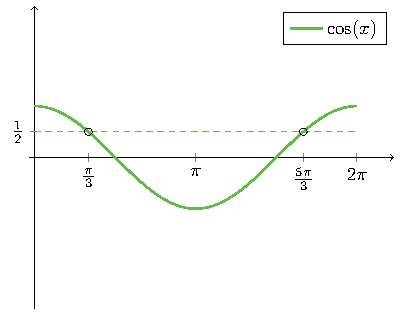
\includegraphics[width=\linewidth]{tut01-umrechnungen-abb-cos} 
			
			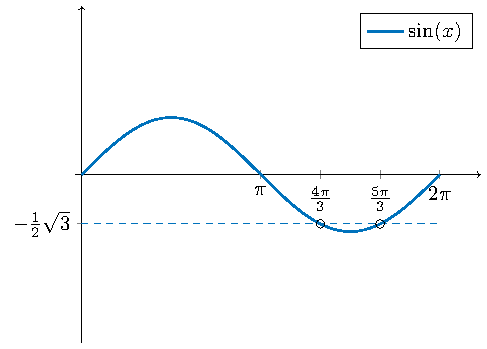
\includegraphics[width=\linewidth]{tut01-umrechnungen-abb-sin}
		\end{minipage}		
		
		Also gilt zusammengefasst:
		\begin{equation*}
			\cos(\phi) = \frac{a}{r} = \phantom{-}\frac{1}{2} \follows \phi \in \menge{\frac{\pi}{3}, \frac{5\pi}{3}} 
			\quad \text{ und } \quad
			\sin(\phi) = \frac{b}{r}  = -\frac{\sqrt{3}}{2} \follows \phi \in \menge{\frac{4\pi}{3}, \frac{5\pi}{3}}
		\end{equation*}
		Da $\phi$ beide Gleichungen erfüllen muss, ist $\phi = \frac{5\pi}{3}$, denn nur der Wert kommt in beiden Lösungsmengen vor.
		Also erhalten wir in Polarkoordinaten
		\begin{equation*}
			z = 2 * e^{\frac{5\pi}{2} \i} 
			\quad \text{ bzw. } \quad 
			z = 2 * \brackets{\cos\brackets{\frac{5\pi}{3}} + \i * \sin\brackets{\frac{5\pi}{3}}}
		\end{equation*}

		\begin{center}
			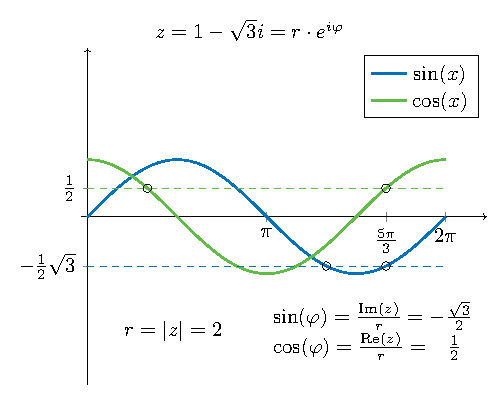
\includegraphics[scale=1]{aufgabe4a-i-bild1}
			\captionof{figure}{Bestimmung des Arguments $\phi = \Arg(z)$}
		\end{center}
	\end{beispiel}

	\pagebreak
	
	\subsection*{Methode 2 --- mit einer kleinen Vorüberlegung}
	Bei dieser Variante machen wir uns vorher kurz Gedanken, wo die komplexe Zahl in der \textsc{Gauß}schen Zahlenebene liegt und was das für den Winkel $\phi$ bedeutet. 
	
	Die Berechnung des Radius bleibt wie oben. 
	Wir überlegen uns anhand der arithmetischen Darstellung, in welchem Quadranten unsere komplexe Zahl liegt.
	\begin{center}
		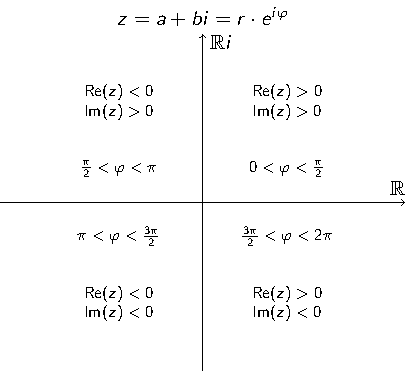
\includegraphics{complex-numbers-angle}
		\captionof{figure}{Zusammenhang zwischen Winkel $\phi$ und Lage der komplexen Zahl in der Ebene}
	\end{center}
	Nun sind Winkel in der Mathematik immer gegen den Uhrzeigersinn gerichtet, d.h. alle Zahlen im ersten Quadranten haben einen Winkel zwischen $0^\circ$ und $90^\circ$ bzw. zwischen $0$ und $\frac{\pi}{2}$. Die weiteren Bereiche sind der Grafik zu entnehmen.
	
	\begin{beispiel}[Aufgabe 4a]
		Die Zahl $z = 1 - \sqrt{3} \i$ hat $\Re(z) = 1 > 0$ und $\Im(z) = - \sqrt{3} < 0$ und muss demnach im 4. Quadranten (rechts unten) liegen. Daher muss der Winkel $\phi$ zwischen $\frac{3\pi}{2}$ und $2\pi$ liegen.
		Wissen wir diese Einschränkung, reicht es aus, wenn wir \textit{eine} der beiden Gleichung 
		\begin{equation*}
			\cos(\phi) = \frac{a}{r} = \phantom{-}\frac{1}{2} 
			\quad \text{ oder } \quad
			\sin(\phi) = \frac{b}{r}  = -\frac{\sqrt{3}}{2}
		\end{equation*}
		lösen. Dabei müssen wir aber darauf achten, genau die Lösung von beiden zu nehmen, die auch wirklich in unserem Zielbereich für $\phi$ liegt.
		Lösen wir also $\cos(\phi) = \frac{1}{2}$, so erhalten wir die Lösung $\frac{\pi}{3}$, die nicht zwischen $\frac{3\pi}{2}$ und $2\pi$ liegt. Daher nehmen wir also die andere, nämlich $\phi = \frac{5\pi}{3}$. 
		\begin{center}
			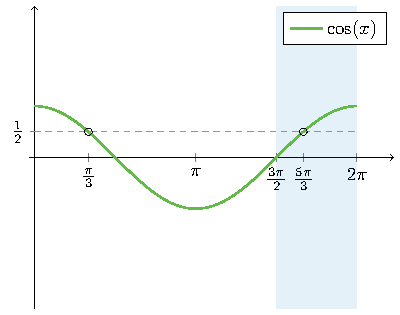
\includegraphics{tut01-umrechnungen-abb-winkelbereich}
			\captionof{figure}{Ein gültiges $\phi$ muss im blauen Bereich liegen.}
		\end{center}
	\end{beispiel}
	
	Wir können die Beobachtung sogar in eine Formel zur Berechnung von $\phi$ zusammenschrumpfen:
	\begin{tcolorbox}[colback=cdorange!10,colframe=cdorange]
		\begin{equation*}
			\phi = \begin{cases}
				\arccos\brackets{\frac{a}{r}} &\text{für } b \ge 0 \\
				2\pi - \arccos\brackets{\frac{a}{r}} &\text{für } b < 0 
			\end{cases}
		\end{equation*}
	\end{tcolorbox}
	wobei der Arkuskosinus immer den Wert zwischen $-\frac{\pi}{2}$ und $\frac{\pi}{2}$ auswirft, weshalb wir für negative Imaginärteile den Winkel noch mit $2\pi$ in den gültigen Bereich verschieben mussten. 
	
	\begin{bemerkung}
		Der Arkuskosinus ist auf vielen Taschenrechnern unter $\cos^{-1}$ zu finden. Analog kann man sich das natürlich auf die den Sinus überlegen.
	\end{bemerkung}
	
\end{document}

